\begin{figure*}[t] % [H] 强制图片在代码位置出现，慎用，有时会影响排版
    \centering % 使整个图表居中
    \captionsetup{skip=-2pt} 
    \setlength{\belowcaptionskip}{-10pt} % 减小主标题与下方正文之间的间距，可调整
    \begin{subfigure}[b]{0.32\textwidth} % [b] 底部对齐，0.32\textwidth 表示每个子图占据文本宽度的32%
        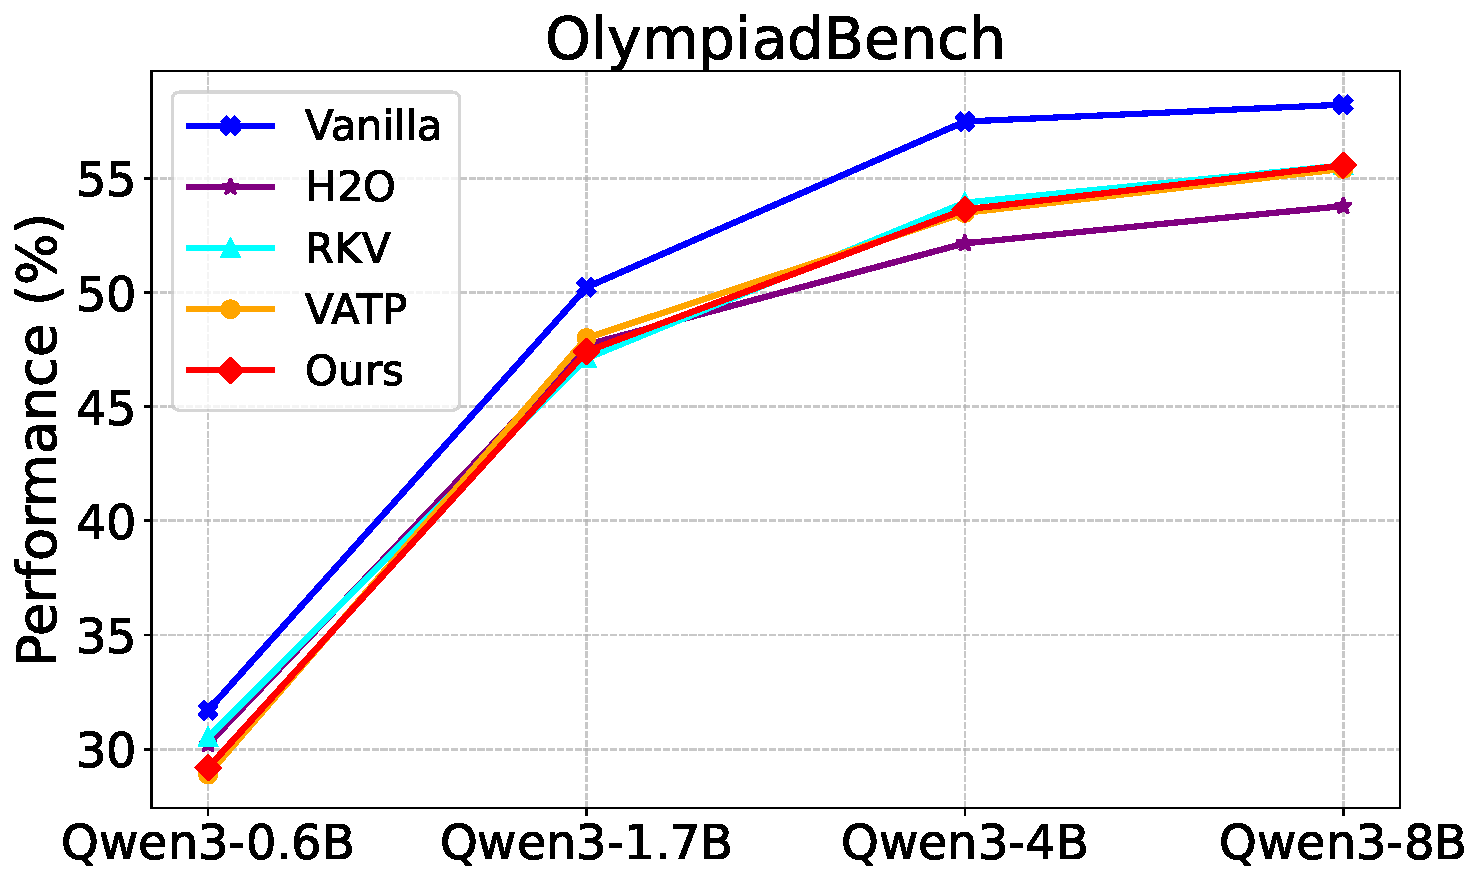
\includegraphics[width=\textwidth]{figure/experiment_different_dataset/qwen_model_OlympiadBench.pdf} % image1.png 是你的图片文件名
        % \caption{Caption for Image 1} % 子图标题 (已注释)
        \label{fig:sub1} % 子图引用标签
    \end{subfigure}
    \hfill % 在子图之间添加水平间距
    \begin{subfigure}[b]{0.32\textwidth}
        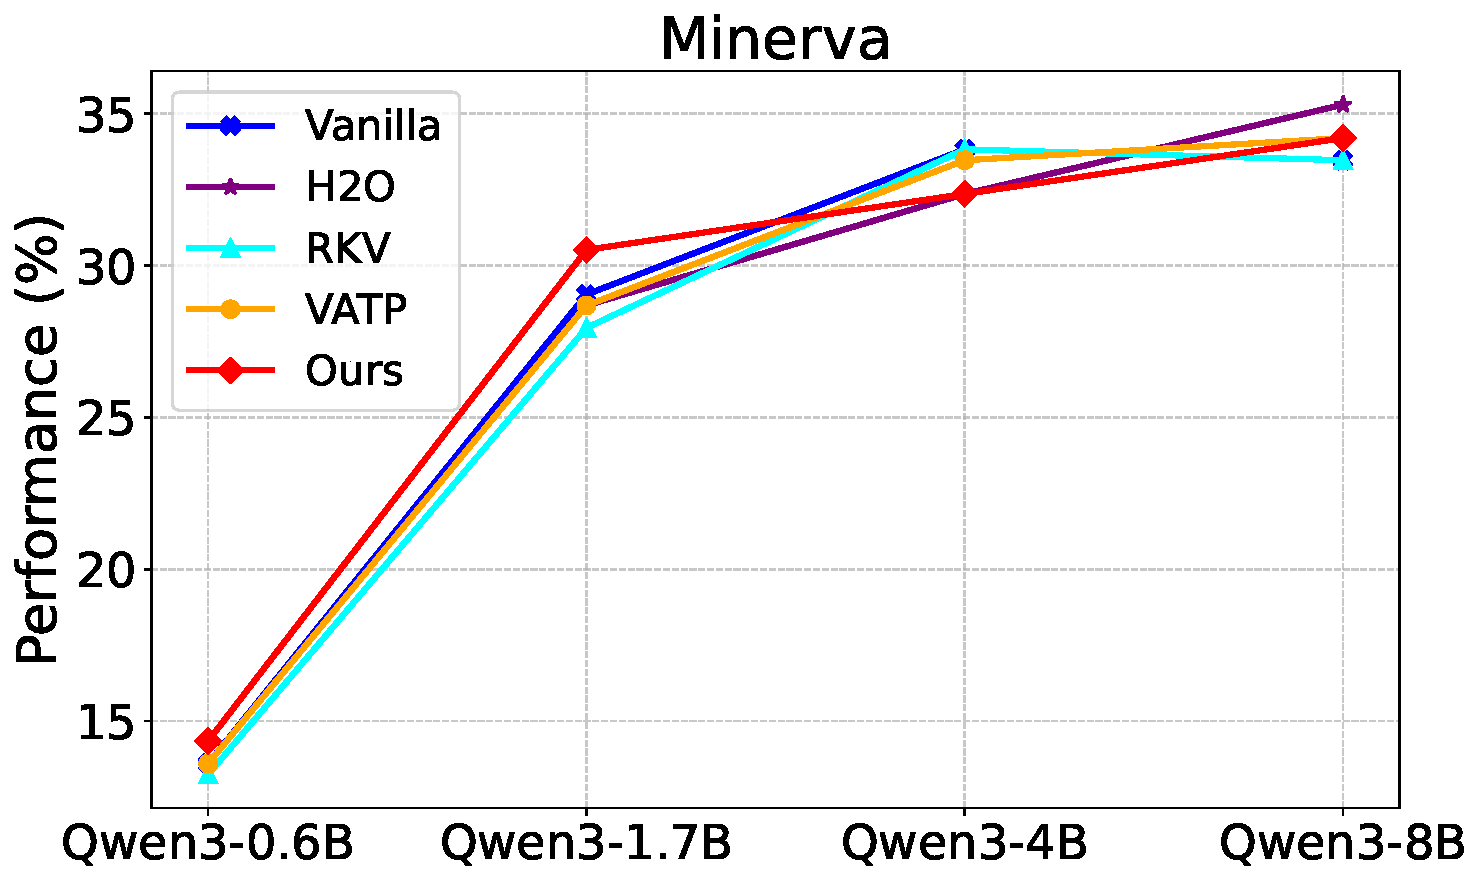
\includegraphics[width=\textwidth]{figure/experiment_different_dataset/qwen_model_Minerva.pdf}
        % \caption{Caption for Image 2}
        \label{fig:sub2}
    \end{subfigure}
    \hfill
    \begin{subfigure}[b]{0.32\textwidth}
        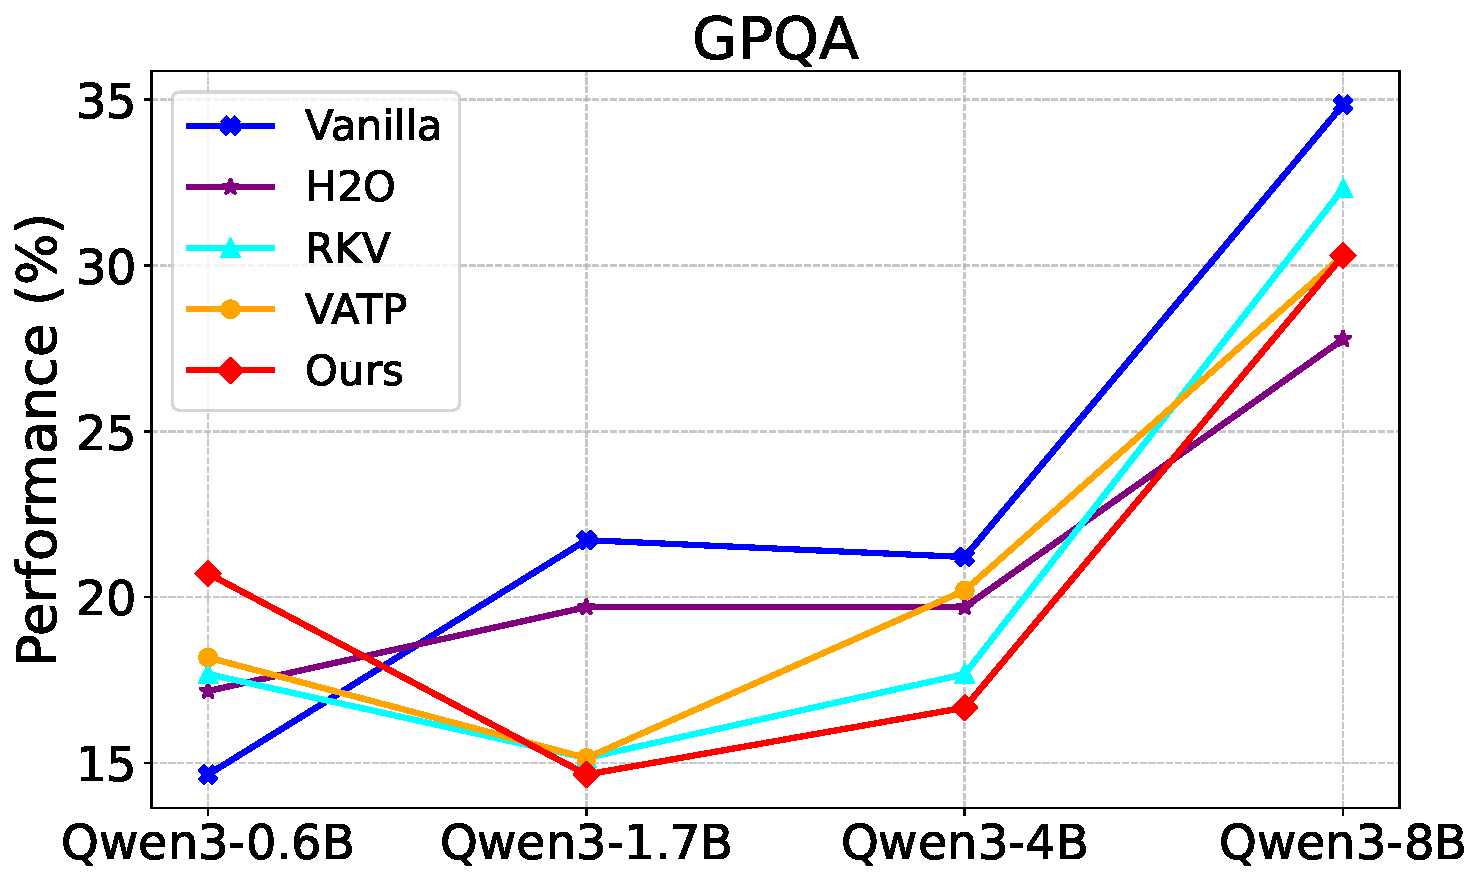
\includegraphics[width=\textwidth]{figure/experiment_different_dataset/qwen_model_GPQA.pdf}
        % \caption{Caption for Image 3}
        \label{fig:sub3}
    \end{subfigure}
    % ----------------------------------------------------------------------------------
    % 关键修改：通过负间距减少两行子图之间的垂直距离。
    % [-1.5em] 是一个常用的起始值，你可以根据实际效果调整，例如 -1em, -2em, -10pt 等。
    % ----------------------------------------------------------------------------------
    \\[-1em] 

    % 第二行
    \begin{subfigure}[b]{0.32\textwidth}
        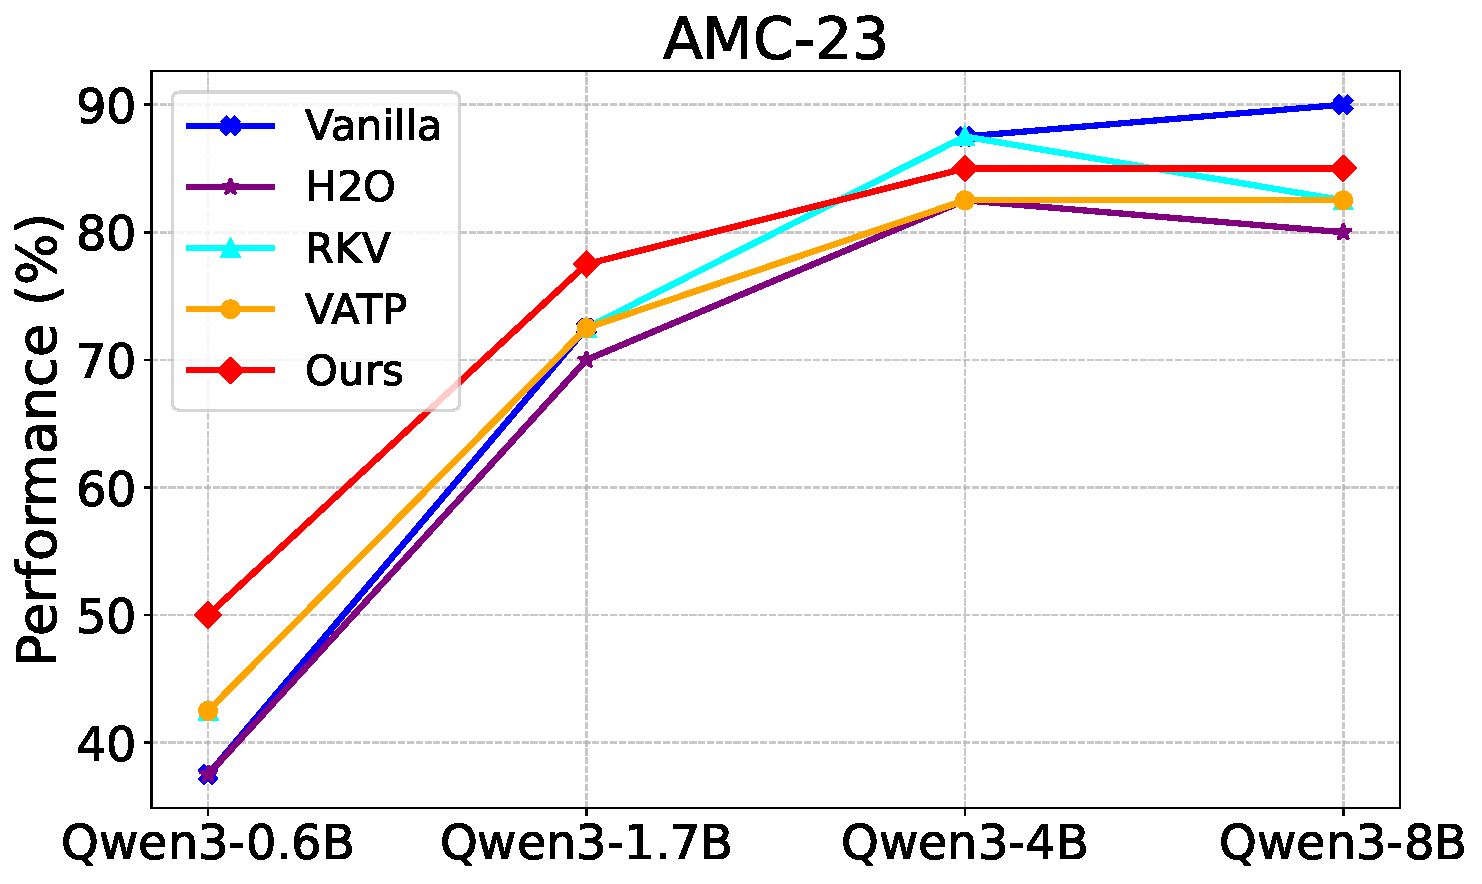
\includegraphics[width=\textwidth]{figure/experiment_different_dataset/qwen_model_AMC-23.pdf}
        % \caption{Caption for Image 4}
        \label{fig:sub4}
    \end{subfigure}
    \hfill
    \begin{subfigure}[b]{0.32\textwidth}
        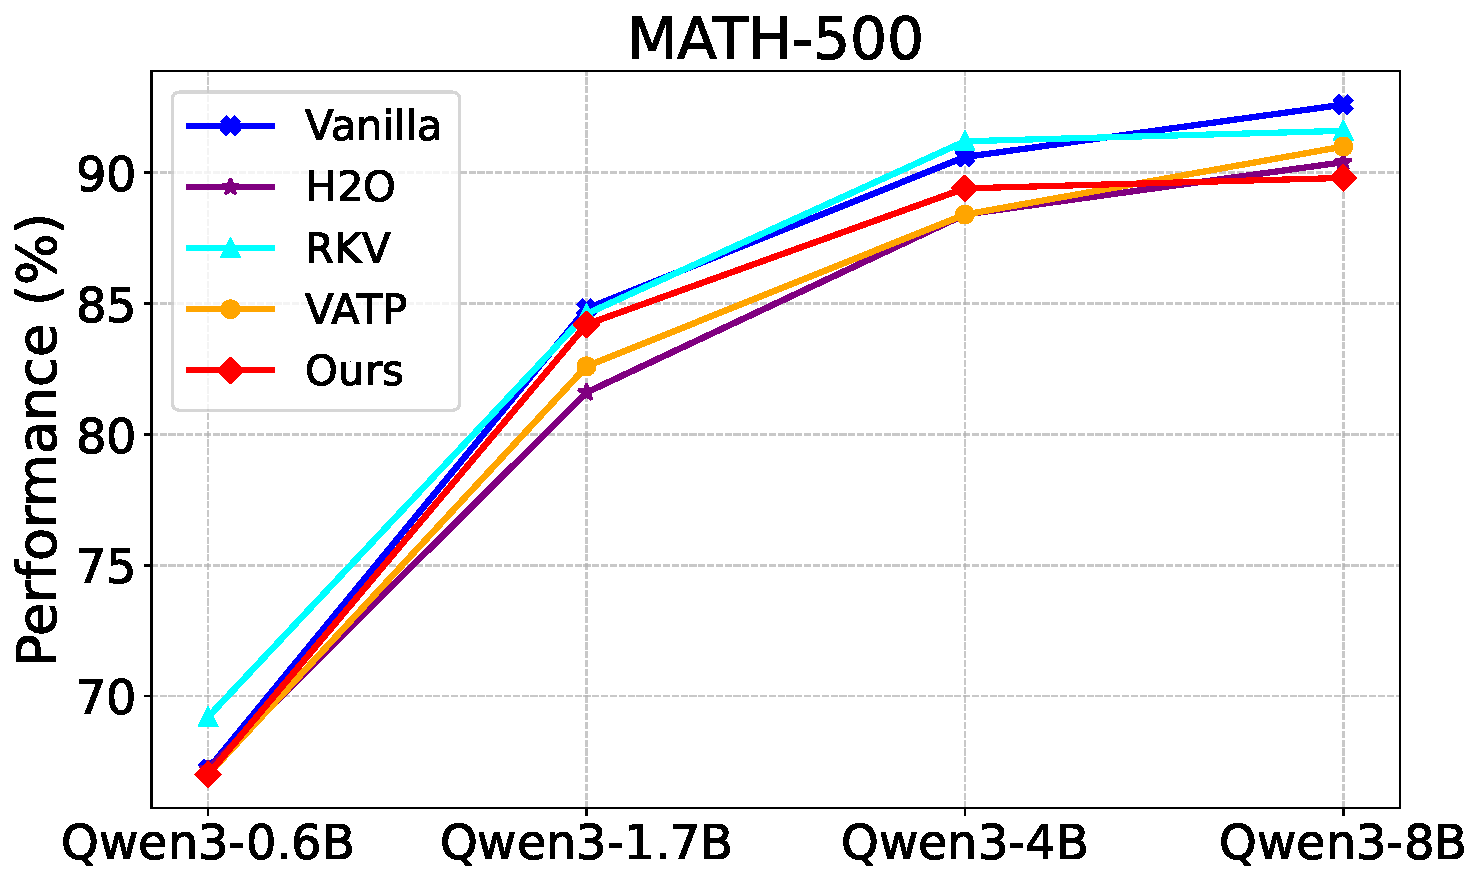
\includegraphics[width=\textwidth]{figure/experiment_different_dataset/qwen_model_MATH-500.pdf}
        % \caption{Caption for Image 5}
        \label{fig:sub5}
    \end{subfigure}
    \hfill
    \begin{subfigure}[b]{0.32\textwidth}
        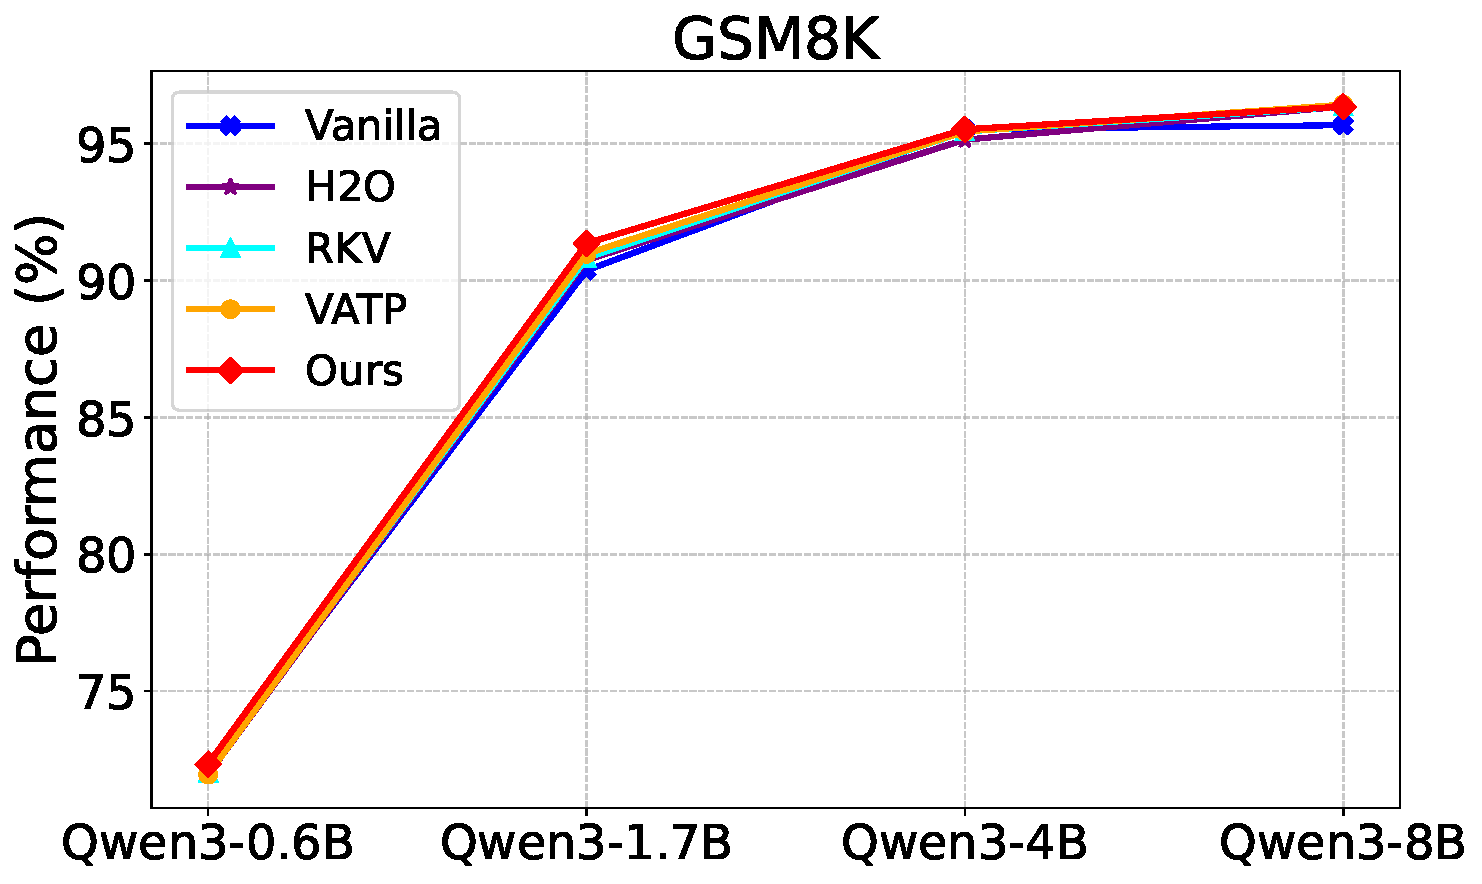
\includegraphics[width=\textwidth]{figure/experiment_different_dataset/qwen_model_GSM8K.pdf}
        % \caption{Caption for Image 6}
        \label{fig:sub6}
    \end{subfigure}
    \caption{Accuracy of LongFlow and the baselines across different model sizes on different datasets.} % 主图标题
    \label{fig:all_images} % 主图引用标签
\end{figure*}
